\section{Codificador 4 a 2 \label{sec:s4}}

\begin{center}
	\begin{minipage}{12cm}
		\begin{tcolorbox}[title=Actividad 4]
			Completar el código del codificador o encoder 4 a 2 en el lenguaje de su elección. Compilar y simular. Configurar en la tarjeta DE2-115, asignar interruptores como entradas y LED´s para observar la salida.
		\end{tcolorbox}	
	\end{minipage}
\end{center}

La visualización RTL del codificador 4 a 2 en Verilog se muestra en la \autoref{fig:encoder_4_2_rtl}. Como se observa, la implementación del codificador 4 a 2 se hace utilizando una instancia de decodificador junto con dos compuertas OR, conectadas de tal forma que corresponden a los dos bits de la salida. Las simulaciones para el código en Verilog se visualizan en la \autoref{fig:encoder_4_2_WaveBi} en base binaria y en la \autoref{fig:encoder_4_2_WaveDe} en base decimal. Se utilizaron todos los valores posibles en las entradas para observar un comportamiento completo en la salida.

\begin{figure}[ht]
	\centering
	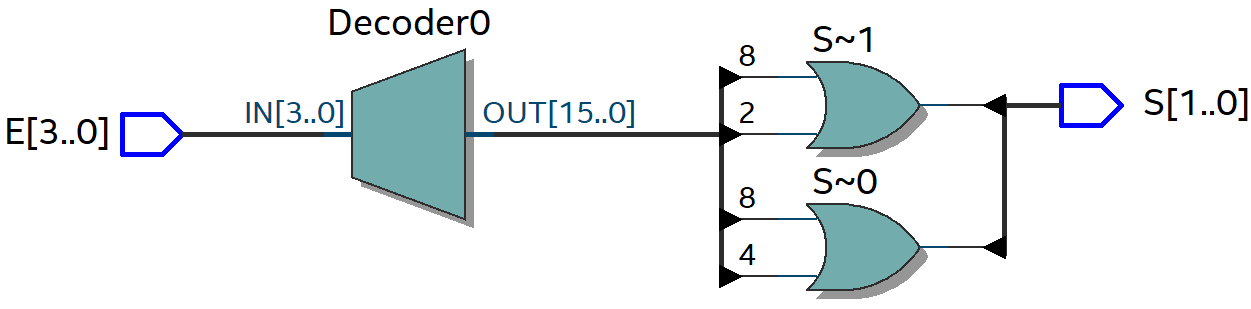
\includegraphics[scale=0.5]{Encoder_4_2_RTL.png}
	\caption{Diagrama RTL del codificador 4 a 2. \label{fig:encoder_4_2_rtl}}
\end{figure}

\begin{figure}[ht]
	\centering
	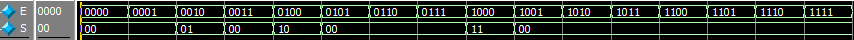
\includegraphics[scale=0.75]{Encoder_4_2_WaveBi.png}
	\caption{Simulación del codificador 4 a 2 con el visor de formas de onda de ModelSim (Base binaria). \label{fig:encoder_4_2_WaveBi}}
\end{figure}

\begin{figure}[ht]
	\centering
	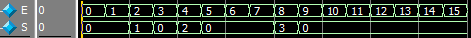
\includegraphics[scale=1.4]{Encoder_4_2_WaveDe.png}
	\caption{Simulación del codificador 4 a 2 con el visor de formas de onda de ModelSim (Base decimal). \label{fig:encoder_4_2_WaveDe}}
\end{figure}